
%mainfile: Multimodal_learning.tex

\begin{titlepage}

  \centering

  \vspace*{1.5em}
  {\LARGE \scshape École Normale Supérieure \par}
  {\Large \scshape Département d'Informatique \par}

  {\Large \scshape Rapport de Stage de L3 \par}

  \vspace{14em}
  {\huge \bfseries Multimodal Learning \par} 
  {\Large \bfseries
    Examples in Gesture and Audio-Visual Speech Recognition \par}

  \vspace{4em}
  {\Large \scshape Hsieh Yu-Guan \par}
  
  \vspace{2em}
  {\Large Sous la direction de \par}

  \vspace{0.5em}
  {\Large \scshape Mathieu Lefort$^1$ \& Amélie Cordier$^2$ \par}

  \vspace{0.5em}
  {\large $^1$LIRIS, Équipe SMA \par}
  {\large $^2$Hoomano, Équipe R\&D \par}

  \vspace{8em}
  {\Large 14 Juin 2017 -- 11 Août 2017}

  \vfill

\end{titlepage}

\section{Introduction} \label{section:introduction}

\subsection{Environment, material and software framework}

Mon stage s'inscrit dans le cadre du laboratoire commun BEHAVIORS.AI
qui est un projet de recherche collaboré entre la société Hoomano et LIRIS.
Hoomano est une entreprise créée en 2014 dédiée au développement de
logiciel de robots sociaux (ex: Nao et Pepper) et son moteur d'interaction
vise à offrer une interaction homme-robot la plus naturelle possible.
Le LIRIS (Laboratoire en InfoRmatique, Image et Système d'Information)
est une unité mixte de recherche en informatique situé à Lyon qui compte
14 équipes de recherche et 330 membres.

Pendant mon stage, j'ai passé les deux premières semaines au
laboratoire et pour le reste du temps j'étais à Hoomano car j'entrînais
les modèles sur le serveur de l'entreprise. Tous les codes ont été
réalisés en python et précisément à l'aide de la biblithèque open source
TensorFlow développé par Google. Cela incluait la construction des
différents architectures et réseaux de neurones, l'entraînement et
l'évaluation.
TensorBoard était un outil assez pratique pour visualiser l'apprentissage,
et je pouvais même facilement visualiser les données et les
représentation apprises grâce au plugin qui est offert.
Toute la suite du rapport sera rédiger en anglais dû à la difficulté
de traduire tous les terms techniques en français.

\subsection{Scientific overview}

Historically, expert systems have been widely used for the design
of artificial intelligence. 
Agents rely heavily on handcrafted ontologies and symbolic rules to
make decisions and act in the world.
Although impressive results have been obtained with this line of
research, it requires a lot of engineering efforts and human knowledge.
Furthermore, engineering in this way all the behaviors that are needed
to display general human level intelligence is out of reach.

On the other hand, we face also the symbol grounding problem
\cite{S. Harnad 1990}. The symbols manipulated by the AI systems have
no meaning to them. To solve these problems, the embodied paradigm
\cite{A. Clark 1997} first argues an agent must be able to perceive and
act from its own perspective (for example, it should be a robot).
Developmental robotics \cite{J. Weng 2001} further emphasizes the
importance of endowing the robot with the capacity of learning new
knowledge from its own sensorimotor experience.

In \cite{L. Smith 2005}, Smith and Gasser discerned six fundamental
principles for the development of emboded intelligence: mulimodality,
incremented development, physical interaction with the environement,
exploration, social guidance and symbolic language aquisition.
I was particularly insterested in the multimodal point in my internship.
The everyday concept that a human acquires is intrinsically multimodal.
For example, the word ``cat'' can be quickly associated with the
appearance of a cat, its vocalization, and the tactile feeling that
we have while petting a cat. The existence of neurons that receive
early information from different modalities have also been proven
\cite{S. Molholm 2002}.

On the other hand, recently, deep learning has achieved a great success in
various domains, such as image recognition \cite{A. Krizhevsky 2012},
text generation \cite{A. Graves 2013} or
machine translation \cite{I. Sutskever 2014}.
It has also been more and more often applied to mutlimodal input
\cite{J. Ngiam 2011, T. Baltrusaitis 2017}.
Its capacity of learning a hierarchical representation of data in a
fully unsupervised way \cite{P. Vincent 2010, A. Radford 2015}
is particularly interesting in the domain of robotics.

In my internship, I studied mainly the application of multimodal learning
using deep networks in the fields of multimodal gesture recognition
and audio-visual speech recognition (AVSR).
I focused especially on the problem
of shared representation learning and knowledge transfer. I wanted to show
that the availablity of multiple modalities could enable the model
to learn a better representation for each single modality and that one can
leverage information from one modality to be used for another when there
is an imbalance of amount of data among different sources.

The report is organized as follow. In Section \ref{section:related} I
briefly review related work on multimodal machine learning, gesture
recognition and AVSR. In section \ref{section:networks}, I present
several basic deep neural network architectures that played an important
role in my work. In section \ref{section:dataset} and
\ref{section:exp}, I describe respectivly the datasets and common
experimental setups that were used in my internship. Experimental
details and results are given in section \ref{section:uni} and
section \ref{section:multi}. Finally, conclusions and perspectives are
presented in section \ref{section:conclusion}.

\section{Related Work} \label{section:related}

\subsection{Multimodal learning}

\cite{T. Baltrusaitis 2017} offers an overview of recent advances in
multimodal machine learning. In \cite{J. Ngiam 2011}, the authors
use a deep network to learn a joint representation of visual and auditory
input. They show that better features for one modality can be learned if
multiple modalities are present at feature learning time. 
There has also been a surge of interest in the exploitation of multimodal
information in the fields of image annotation \cite{J. Weston 2010},
zero-shot learning \cite{A. Frome 2013, R. Socher 2013}, and automatic
image caption generation \cite{A. Karpathy 2015}. They first train
visual and language models separately and as a next step they try
to learn either a common embedding \cite{J. Weston 2010}, a mapping
\cite{A. Frome 2013, R. Socher 2013} or an alignment \cite{A. Karpathy 2015}
between the two models.

Applications in the field of robotics can also been found.
\cite{A. Droniou 2014} proposes a network that is able to learn both
a symbolic representation of data and a fine discrimination between
two similar stimuli in an unsupervised way. The authors apply their method
to visual, audiotory and proprioceptive data of the humanoid robot iCub.
A multimodal embedding that is able to combine information coming from
vision, language and motion trajectories is defined in \cite{J. Sung 2017}
and endows the robot with the capacity of manipulating a unseen object.

\subsection{Gesture recognition}

Gesture recognition has been studied for a while within the fileds of
computer visoin and pattern recognition
\cite{T. Starner 1998, S. Mitra 2007}.
Recently, deep learning algorithms have led to
significant advances in this domain \cite{M. Asadi-Aghbolaghi 2017}.
The use of Convolutional Neural Networks (CNNs) is the most common
\cite{J. Nagi 2011}. 3d CNNs are used to deal with image sequences in
\cite{P. Molchanov 2015}. Architectures that take in multimodal inputs
have also grown in popularity. \cite{N. Neverova 2013} copes with color,
depth, skeleton and audio information using CNNs and Recurrent
Neural Networks (RNNs). Others use 3d CNNs and deep belief networks
(DBNs) while facing similar multimodal inputs
\cite{N. Neverova 2014, L. Pigou 2014, D. Wu 2016}.

\subsection{Audio-visual speech recognition}

AVSR is probably one of the earliest examples of multimodal research.
Most early works were based on various hidden Markov model (HMM) extensions
\cite{G. Potamianos 2004}, but the use of neural networks were also
explored \cite{C. Bregler 1994, B. P. Yuhas 1989}. Although research
into AVSR is not as common these days, it has drawn attention from the
deep learning community
\cite{J. Ngiam 2011, K. Noda 2014, A. K. Katsaggelos 2015}.
A transfer deep learning framework applied in AVSR proposed in
\cite{S. Moon 2015} forms the base of my study in
\ref{subsection:AVSR_transfer}. \cite{L. Deng 2013} and
\cite{G. Hinton 2012} give several examples of how deep architectures can
be used to deal with audio data.

\section{Presentation of Basic Network Architectures}
\label{section:networks}

\subsection{Convolutional Neural Network}

CNNs are an early family of deep learning
architectures inspired from the human vision system \cite{Y. LeCun 1998}.
Generally we have convolutional layers alternating with pooling
(subsamping) layers, but fully connected layers can also be introduced.
CNNs have been shown to achieve state-of-the-art performance in
image processing tasks such as image classification
\cite{A. Krizhevsky 2012} and object detection \cite{Y. LeCun 2010}.
However they can be equally applied in other fields like speech recogntion
\cite{L. Deng 2013}.

For a convolutional layer with a mono-channel input $x$, the latent
representation of the k-th feature map is given by

\[h^k = \sigma(x\ast W^k + b^k)\]

where $W^k$ is the k-th kernel, $b^k$ the bias is broadcasted to the whole
feature map, $\ast$ denotes the 2d convolution and $\sigma$ is an
ativation function. When there are multiple input channels, the kernel
is extended to the full depth of input. In TensorFlow, two different
zero paddings are defined, `SAME' and `VALID'. For `SAME' padding,
$height_{out} = \lceil height_{in}/strides[1] \rceil$,
and for `VALID' padding,
$height_{out} = \lceil (height_{in}-height_{filter}+1)/strides[1] \rceil$.
It's similar for the width.

The TensorFlow page: 
\href{https://www.tensorflow.org/api_guides/python/nn#Convolution}
{https://www.tensorflow.org/api\_guides/python/nn\#Convolution}.

In \cite{S. Ji 2013}, 3d CNNs are proposed to be used for video inputs.
They're like traditional CNNs except for the fact that we replace
2d feature maps by 3d feature maps and 2d kernels by 3d kernels.

\subsection{Auto-Encoder} \label{subsection:AE}

Auto-Encoders are networks that are trained to minimize the reconstruction
error by back-propagating it from the output layer to hidden layers.
In the simplest model with one hidden layer, an auto-encoder takes an
input $\mathbf{x} \in \mathbb{R}^d$ and maps it to the latent
representation $\mathbf{h} \in \mathbb{R}^{d'}$ given by
$\mathbf{h} = \sigma(W\mathbf{x}+\mathbf{b})$ where $W$
is a weight matrix, $\mathbf{b}$ is a bias vector and $\sigma$ is an
activation function. Then the network tries to reconstruct the input
by a reverse mapping $\mathbf{x'} = \sigma(W'\mathbf{h}+\mathbf{b'})$.

To prevent the auto-encoder from learning the identity function as
a trivial solution, several regularization techniques have been proposed.
The bottleneck approach forces dimensionality reduction by having
fewer neurons in hidden layers than in the input layer. For example,
in the above case, we must have $d'<d$. Sparse auto-encoders impose sparsity
on hidden units \cite{A. Makhzani 2014}.
Denoising auto-encoders, which play an important role in my internship,
try to recontruct the clean input from its corrupted version
\cite{P. Vincent 2008, Y. Bengio 2012}. Binomial noise
(switching pixels on or off) adding
to input or hidden layers are used in my case.

Intuitively, auto-encoders are useful for data reconstruction.
Nevertheless, the true interest lies in fact in its capcity to learn
a representation (encoding) for a set of data in a purely unsupervised
fashion \cite{P. Vincent 2010}. Recently, auto-encoders are also
more and more often used as a generative model \cite{Y. Bengio 2013}.

\subsection{Convolution Auto-Encoder}

Fully connected auto-encoders ignore the 2d image structure.
This can cause problems when dealing with real-world size inputs,
and introduces redundancy in the parameters.
Convolutional Auto-Encoders \cite{J. Masci 2011, V. Turchenko 2017}
(CAEs) are intuitively similar
to architectures described in \ref{subsection:AE}.
However, convoluitonal and transposed convolutional layers are used instead.
Transposed convoluitonal layers are also called deconvolutional
layers \cite{M. D. Zeiler 2011}.
We perform in fact also a convolution operation but with zero paddings
around the image and sometimes around each pixel to upsample the
image and to inverse the previous convolution
(imagine that if the value of one pixel comes from 9 pixels of the
previous layer, when doing a transposed convolution this pixel
contributes to the same 9 pixels for reconstruction).
This github directory
\href{https://github.com/vdumoulin/conv_arithmetic}
{https://github.com/vdumoulin/conv\_arithmetic}
is quite useful for the understanding of the concept.

Pooling and unpooling layers are also sometimes considered in a CAE
architecture \cite{V. Turchenko 2017}. As they weren't used
in my architecture I will not spend time explaining what an unpooling
layer is.

\section{Datasets and Preprocessing} \label{section:dataset}

Many datasets were explored during my internship. The three main datasets
being used are given in details  below. Two of them are for gesture
recognition:
Creative Senz3D \cite{A. Memo 2015, A. Memo 2017} and ASL Finger Spelling
\cite{N. Pugeault 2011}, and one is for AVSR: AVLetters
\cite{I. Matthews 2002}.

\subsection{Creative Senz3D}

The dataset contains gestures perfomed by 4 different people, each
performing 11 different static gestures repeated 30 times each,
for a total of 1320 samples.
For each sample, color, depth and confidence frames are available.
I only used the color and depth frames of this dataset. The original
size of each image is $480 \times 640$ and they're resized to
$299 \times 299$ pixels before being fed to the network. No other
preprocessing are done. For both color and depth images I use the three
color channels (even though a priori only one channel is needed for
depth maps).

\begin{figure}[H]
  \centering
  \hfill
  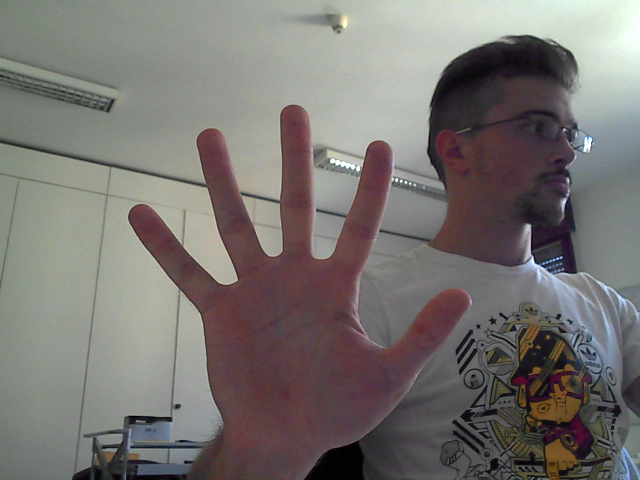
\includegraphics[width=0.23\linewidth]{dataset/senz3d/examples/1-color}
  \hfill
  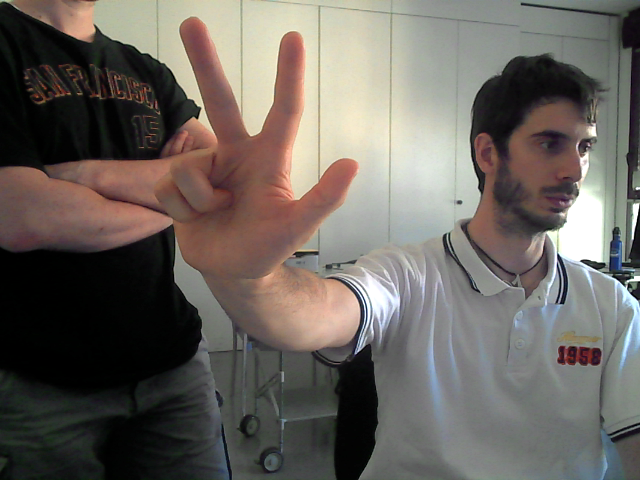
\includegraphics[width=0.23\linewidth]{dataset/senz3d/examples/12-color}
  \hfill
  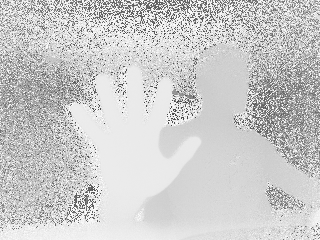
\includegraphics[width=0.23\linewidth]{dataset/senz3d/examples/1-depth}
  \hfill
  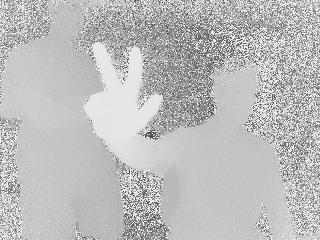
\includegraphics[width=0.23\linewidth]{dataset/senz3d/examples/12-depth}
  \caption{%
    \textbf{Example images in the Creative Senz3D dataset.}\\[0.1em]
    Left Two) Color images.\\[0.1em]
    Right Two) Corresponding depth images.\\[0.1em]
    All of the images are of size $480 \times 640$ and contain the
      the entire upper body of the subject.}
  \label{fig:senz3d_exs}
\end{figure}

\subsection{ASL Finger Spelling}

The dataset is composed of more than 60000 images in each modality
(RGB and depth images are provided).
Five subjects are asked to perform the 24 static signs in
the American Sign Language (ASL) alphabet (excluding j and z which involve
motion) a certain number of times, captured with similar lighting
and background.

Images of this dataset are of variable sizes. The data preprocessing
includes resizing each image to $83 \times 83$ pixels,
converting to grayscale and Z-normalization (normailzing to zero mean
and unit of variance).

\begin{figure}[H]
  \centering
  \hfill
  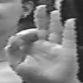
\includegraphics[width=0.23\linewidth]{%
    dataset/fingerspelling5/exs/st/g1}
  \hfill
  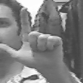
\includegraphics[width=0.23\linewidth]{%
    dataset/fingerspelling5/exs/st/g2}
  \hfill
  
\includegraphics[width=0.23\linewidth]{%
    dataset/fingerspelling5/exs/st/d1}
  \hfill
  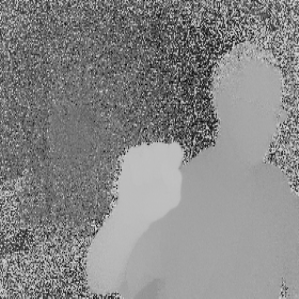
\includegraphics[width=0.23\linewidth]{%
    dataset/fingerspelling5/exs/st/d2}
  \caption{%
    \textbf{Example images in the ASL Finger Spelling dataset
      (after preprocessing).}\\[0.1em]
    Left Two) Grayscale intensity images.\\[0.1em]
    Right Two) The corresponding depth maps.\\[0.1em]
    Images of this dataset have variable sizes, and they're all resized to
      $83 \times 83$ before being fed to the network. Generally only the
      hand region is contained in image.}
  \label{fig:fingerspelling_exs}
\end{figure}

\subsection{AVLetters}

The dataset comprises video and audio recordings of 10 speakers
uttering the letters A to Z, three times each.
We count therefore 780 samples in total. For video data, image sequences
of pre-extracted lip regions are provided.
Each single image if of size $60 \times 80$.
For audio data, only the mel-frequency cepstrum coefficients (MFCCs)
are given, and each audio frame is represented by 26 mfccs.
The lack of raw audio data is a strong constraint on what we're able to do
on this dataset.

Since all utterances don't have the same time duration, I used
fourier resamping to force every video input to be of length 12 and
every audio input to be of length 24. Video frames are Z-normalized.
Several data augmentation techniques
are also considered, including random brightness adjusting, random contrast
adjusting and random cropping (but at least 80\% of the original image
is kept).

\begin{figure}[H]
  \centering
  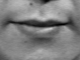
\includegraphics[width=0.15\linewidth]{%
    dataset/avletters/lips_no_data_aug/1}
  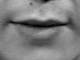
\includegraphics[width=0.15\linewidth]{%
    dataset/avletters/lips_no_data_aug/2}
  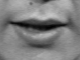
\includegraphics[width=0.15\linewidth]{%
    dataset/avletters/lips_no_data_aug/3}
  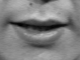
\includegraphics[width=0.15\linewidth]{%
    dataset/avletters/lips_no_data_aug/4}
  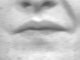
\includegraphics[width=0.15\linewidth]{%
    dataset/avletters/lips_no_data_aug/5}
  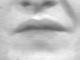
\includegraphics[width=0.15\linewidth]{%
    dataset/avletters/lips_no_data_aug/6}\\[0.15em]
  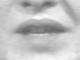
\includegraphics[width=0.15\linewidth]{%
    dataset/avletters/lips_no_data_aug/7}
  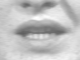
\includegraphics[width=0.15\linewidth]{%
    dataset/avletters/lips_no_data_aug/8}
  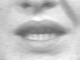
\includegraphics[width=0.15\linewidth]{%
    dataset/avletters/lips_no_data_aug/9}
  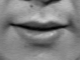
\includegraphics[width=0.15\linewidth]{%
    dataset/avletters/lips_no_data_aug/10}
  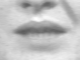
\includegraphics[width=0.15\linewidth]{%
    dataset/avletters/lips_no_data_aug/11}
  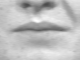
\includegraphics[width=0.15\linewidth]{%
    dataset/avletters/lips_no_data_aug/12}
  \caption{%
    \textbf{Example visual input for the AVletters dataset
      (left to right, top to bottom).}\\[0.1em]
    Pre-extracted lip regions of $60 \times 80$ pixels are provided.
      Each image sequence is resampled to be of length twelve in order to
      give an input of fixed size to the network.}
  \label{fig:avletters_exs}
\end{figure}

\section{Experimental Setup} \label{section:exp}

To train a classifier I employed the cross entropy cost function and to
train an auto-encoder the L2 distance between the input and output vector
was used as the loss. For the sake of preventing overfitting, L2
regularization \cite{Y. Bengio 2012} was applied to all the weights of
network with a regularization coefficient $\eta$.
The Adam algorithm \cite{D. Kingma 2014}
was then introduced for minimizing the loss function.
An exponential decay was further used for the stepsize $\alpha$ of this
algorithm with an initial stepsize $\alpha_0$ varying from 0.01 to 0.0001
depending on experiment. The decaying rate $\gamma$
was generally close to 0.8 and
the decay takes place every 100 training steps.

Inputs of the network were normally fed as mini-batches of size 24
(smaller and bigger batch sizes were also experimented).
Batch normalization \cite{S. Ioffe 2015} were introduced after every
convolutional and transposed convoluitonal layer. Therefore, the real
operations used to compute neural activations are more complicated
then what are described above. The used settings and hyperparameter
values aren't necessarily optimal since I wasn't able to test all the
possible combinations.

Here are some more details of the network architectures: ReLu
(Rectified Linear Unit) activation were added to all the hidden layers
\cite{A. Krizhevsky 2012} while no activation function was used for
the output layer.
For classification model dropout \cite{N. Srivastava 2014}
was always applied to the second to last layer during training.
The output of the classification layer was mapped to the probabilities
that one data example belongs to each class by the softmax function.

For classification experiments, except for the one described in
\ref{subsection:AVSR_transfer}, the dataset was always separated into
training and test set. The classifier was first trained on the training data
and then tested on test data once the training phrase was finished.
Unless stated otherwise, the prediction accuracies mentioned hereinafter
were always evaluated on the test set.

\section{Experiments and Results: Unimodal Cases} \label{section:uni}

\subsection{Classification} \label{subsection:classif}

With every new dataset, I began with training a classifier on it in a
totoally supervised manner.
This gave me an insight into its data quality, the preprocessing
effectiveness and ensured that further experiments could be conducted.
CNN is then one of the most suitable architecture for this purpose.

\subsubsection{Creative Senz3d}

No satisfying results were acquired. It may be due to to a lack of data
quantity, variety, and the fact that the head is also contained in the
image increases significantly the classification difficulty.

\textbf{Subject Dependent.}
In a subject dependant setting, images are separated randomly into
training set (3/4) and test set (1/4). Therefore, during the
testing phase, the classifier doesn't need to deal with data from an
individual that it has never seen before.
In this case, for RGB images, all of the classifiers were able to
have a classification accuracy that is closed to 100\%. This held true
even for a perceptron.
On the other hand, for depth images, the classification accuracy was
between 60\% and 70\% using a perceptron and near 90\% for other CNN
architectures that were tested.

\textbf{Subject Independant.}
On the contrary, the classifier faces individuals never seen before
during testing in a subject independant setting. 
In my case, the training set consisted of images coming from the
first three individuals while the test set contained images of
the final subject.
With the various architectures (including single-layer perceptron
and CNNs varying from three to ten hidden layers)
that I implemented, none of them was able to generalize the learned model
to the new individual.
The pre-trained InceptionV4 architecture \cite{C. Szegedy 2017}
achieved a prediction accuracy
of 30\% for color images and 20\% for depth images (better than chance).

\subsubsection{ASL Finger Spelling} \label{subsubsection:ASL_CNN}

The large number of data contained in this dataset and the relatively
simple image content (single hand instead of the entire upper body)
makes the classification task much easier. By using the CNN architecture
shown in \autoref{fig:CNN10}, I could achieve a classification accuracy
of respectively 80\% and 70\% for intensity and depth images
(\autoref{tab:ASL_classif})
in an subject-independant setting (four subjects for training and one
subject for testing). We may not need that many layers in the CNN
architecture, but further tests were not carried out since it's not
the essential point of my internship.

\subsubsection{AVLetters}

One can refer to \autoref{fig:AVSR_transfer} for the main CNN architectures
that were used in this dataset. 
Notice that 3d CNNs were employed to deal with video inputs.
Considering the small number of available data, a speaker-dependent
setting was used.
With some carefully chosen hyperparameter values and network architectures,
the prediction accracy was of near 80\% for audio and about 55\% for video.

When using CNNs, whether to add the first- and second-order frame-to-frame
differences of MFCCs (\textit{delta} and \textit{delta-delta}) didn't seem
to have a great impact on the final result, so in the latter transfer
learning experiment described in \ref{subsection:AVSR_transfer}, only
MFCCs were fed as input of the network.
Concerning video input, the use of data augmentation techniques only
decreased the learning speed for the training part but didn't improve
the performace for testing.

\begin{figure}[H]
  \centering
  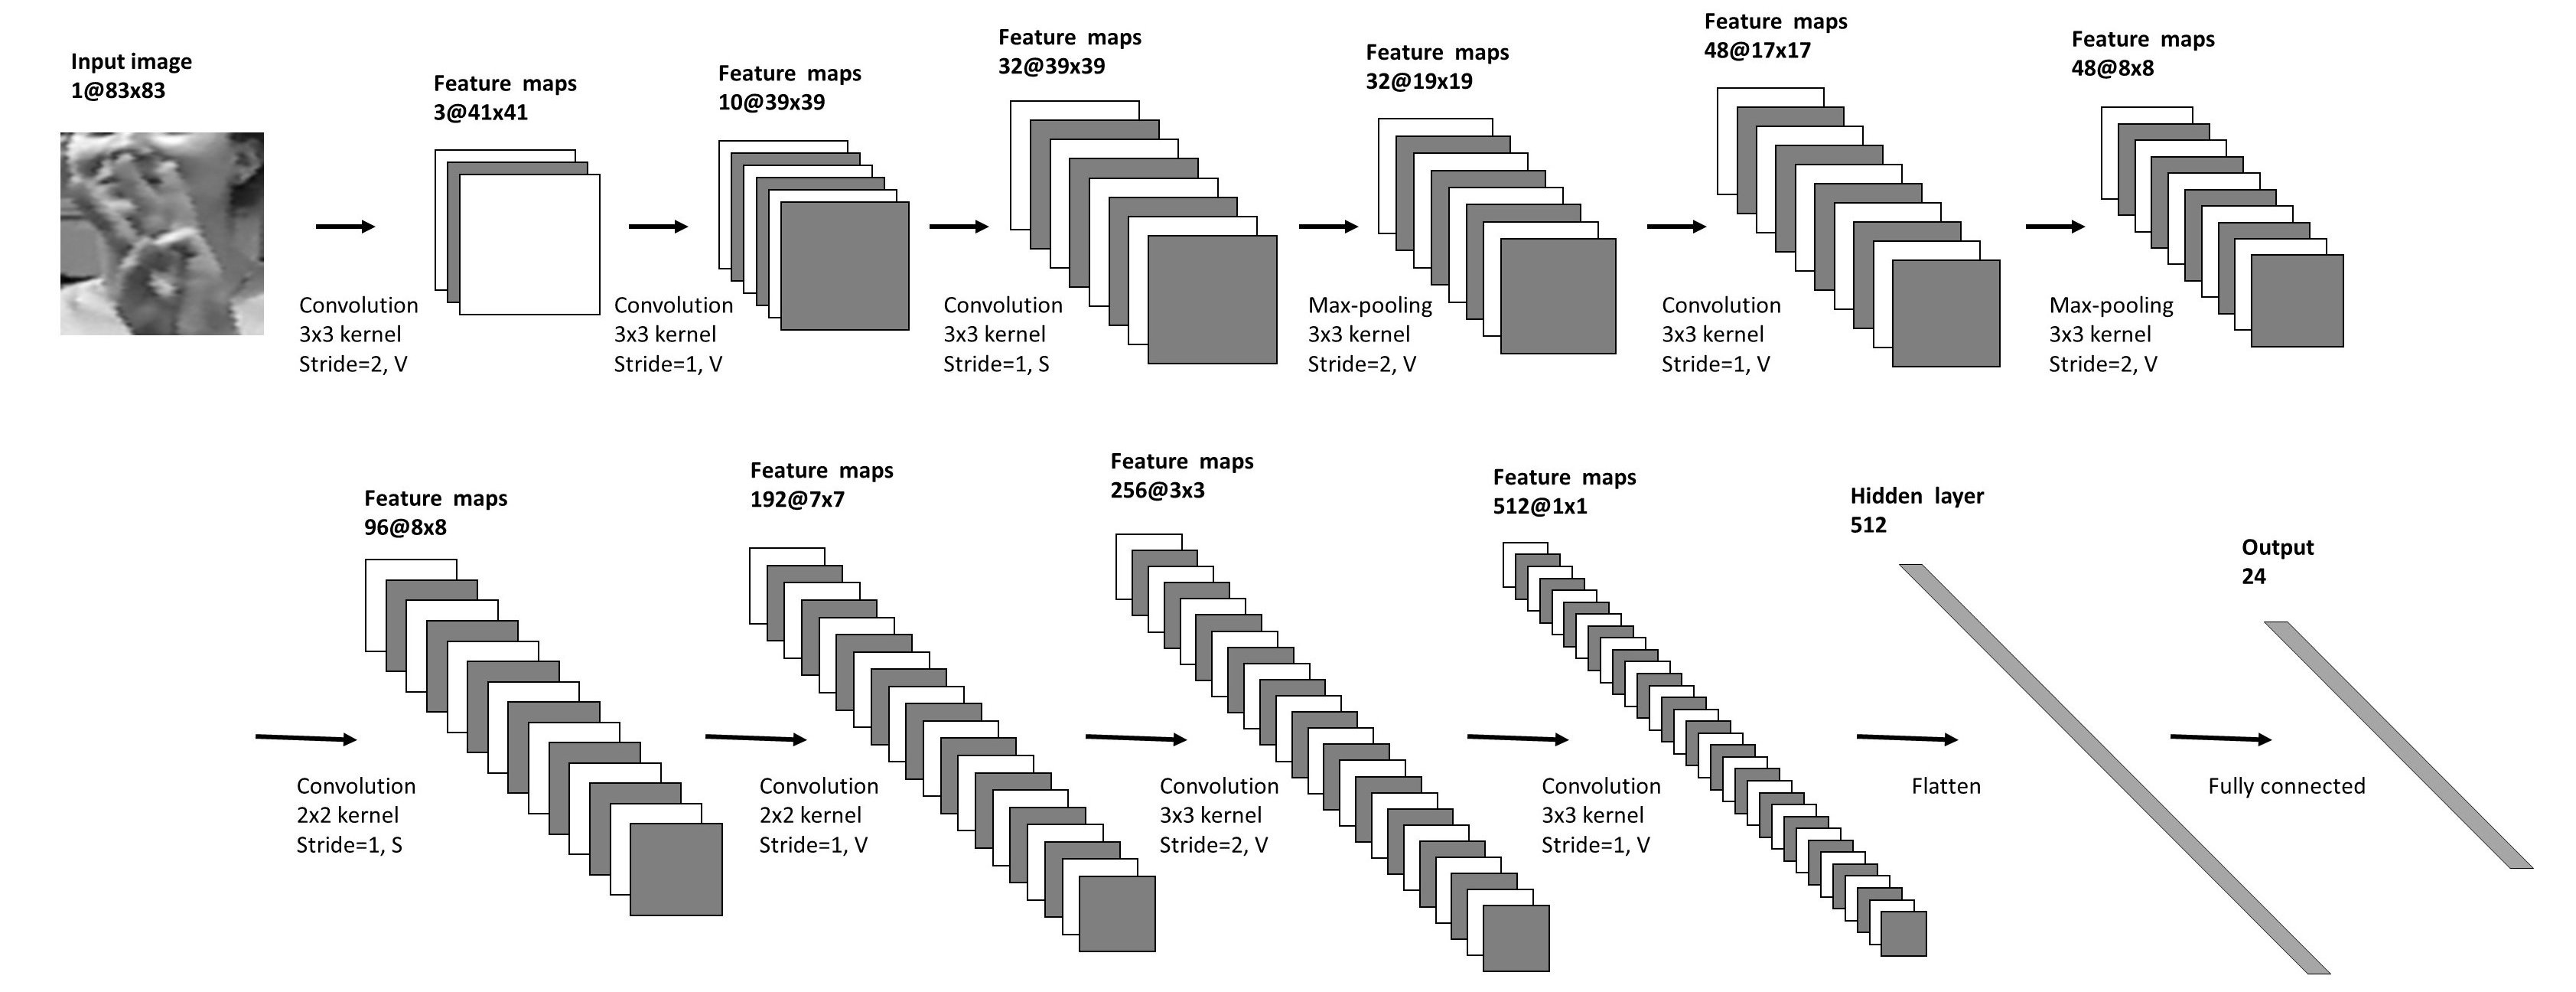
\includegraphics[width=\linewidth]{architectures/CNN10}
  \caption{%
    \textbf{CNN architecture used for the Finger Spelling  dataset.}
      \\[0.1em]
    The input of the nework is a one-channel image of size $83 \times 83$.
      It contains ten hidden layers. S stands for `SAME' padding
      and V stands for `VALID' padding (see text).}
  \label{fig:CNN10}
\end{figure}

\subsubsection{Problem of overfitting}

Overfitting was observed for almost all the classification
experiments, and it was particularly severe for
CNNs with many layers.
In fact, CNN architectures could usually classify
perfectly the training data, but experienced a drop of performance
when evaluating on test set.

It's well known that by reducing the number of hidden layers and
increasing the weight regularization coefficient $\eta$ we may
be able to cure this problem.
For example, when $\eta$ was augmented from $0.0004$ to $0.1$,
the classification accuracy for the audio input of the AVLetters
dataset increased by about 10\%.
By using fewer hidden layers in the 3d CNN architecture overfitting
was also alleviated when dealing with the video input of this same dataset.
However, these techniques didn't always work
and more often I got a poorer performance during training without
an improvement of performance for test.

\subsection{Convolutional auto-encoder} \label{subsection:CAE}

Several distinct CAE architectures were tested in my internship.
Here I present the one with five hidden layers; therefore it contains
three convolutional layers and three transposed convolutional layers
as illustrated in \autoref{fig:CAE5}. The end-to-end training instead of
a greedy layer-wise approach was employed.

The proposed architecture was then trained on the two gesture recognition
datasets. First of all, I was interested in the denoising capcity of
the auto-encoder. An example is given in \autoref{fig:image_restoration}.
The auto-encoder is effectively able to reconstruct the clean image in
a way, even though the result is blurred and sometimes distorted.

What's more important, can meaningful high-level features be
learned in this way? The output of the middle layer was taken as a
new representation of the input data.
By doing principal component analysis, it could be projected into
three dimensions for visualization.
However, to quantify the learned features, they're further used for
classification by training a perceptron on top of it.

As suggested in \ref{subsection:classif}, I used a subject-dependant setting
for Creative Senz3d while a subject-independant setting was employed
for ASL Finger Spelling. I compared this new classifier with a
perceptron built on raw data input. As already mentioned earlier, the
latter could classify perfectly the input when dealing with color images
of Creative Senz3d. In other cases, I observed always an improvement
of 10-20\% for the prediction accuracy thanks to the use of the
learned representation of the data (refer to \autoref{tab:ASL_classif}
for results on ASL Finger Spelling). Useful high-level data representation
can thus be learned in a totally unsupervised manner.

\begin{figure}[H]
  \centering
  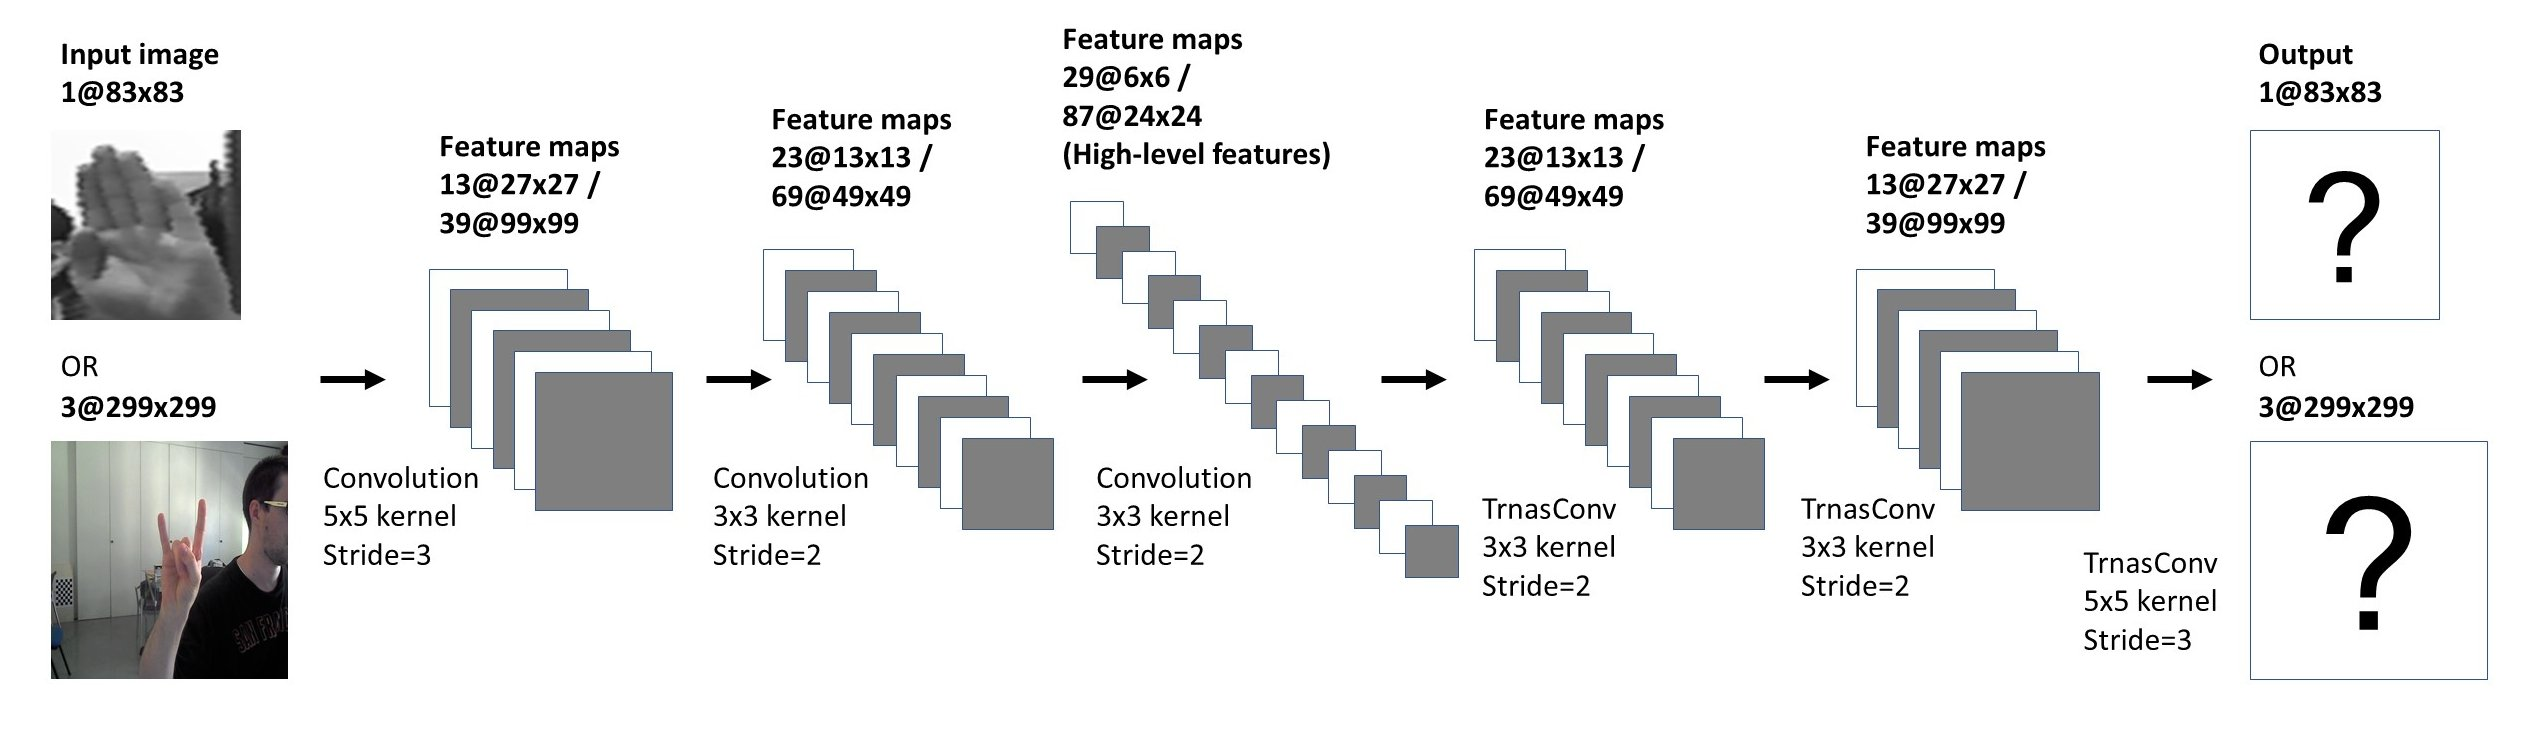
\includegraphics[width=\linewidth]{architectures/CAE5}
  \caption{%
    \textbf{Convolutional auto-encoder architecture with 
      three convolutional layers and three tranposed convolutional
      layer.}\\[0.1em]
    Activation values of the middle layer are taken as 
      high-level features of the input image. Inputs of the network
      can be of different sizes. We only use valid paddings here.}
  \label{fig:CAE5}
\end{figure}

\begin{figure}[H]
  \centering
  \hfill
  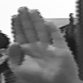
\includegraphics[width=0.28\linewidth]{%
    dataset/fingerspelling5/gray/gray5}
  \hfill
  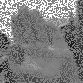
\includegraphics[width=0.28\linewidth]{%
    dataset/fingerspelling5/gray/gray_dropout5}
  \hfill
  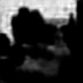
\includegraphics[width=0.28\linewidth]{%
    dataset/fingerspelling5/gray/gray_reconstruction5}
  \caption{%
    \textbf{Image restoration using convolutional auto-encoder.}\\[0.1em]
      Left) Clean Image.\\[0.1em]
      Middle) Noisy image [input].\\[0.1em]
      Right) Restored image [output].}
  \label{fig:image_restoration}
\end{figure}

\section{Experments and Results: Multimodal Cases} \label{section:multi}

\subsection{Shared representation learning} \label{subsection:shared}

A first fundamental chanllenge in multimodal learning is the problem
of representing and summarizing data from several modalities.
How can we relate information from multiple sources?
Mainly inspired from \cite{J. Ngiam 2011, A. Droniou 2014},
I generalized the CAE architecture introuduced in \ref{subsection:CAE}
to a multimodal setup. As presented in \autoref{fig:FAE5}, two CAEs
of different modalities share a common middle layer by doing a sum
of corresponding values. I first pre-train the first two layers
of each modality using an unimodal CAE. In a second stage, I train the
rest of the network to reconstruct the two modalities of the input.

To prevent the network from finding representations such that different
hidden units are tuned for different modalities separately, random
dropouts are added to inputs in such a way that only by combining the
two modalities we have 100\% of the input information. In particular,
sometimes one modality can be totally absent whereas the whole clean
image is given for the other modality. In addition, proper scaling were
also considered to keep the expected sum of the activations at each layer
to be the same.

\begin{figure}[H]
  \centering
  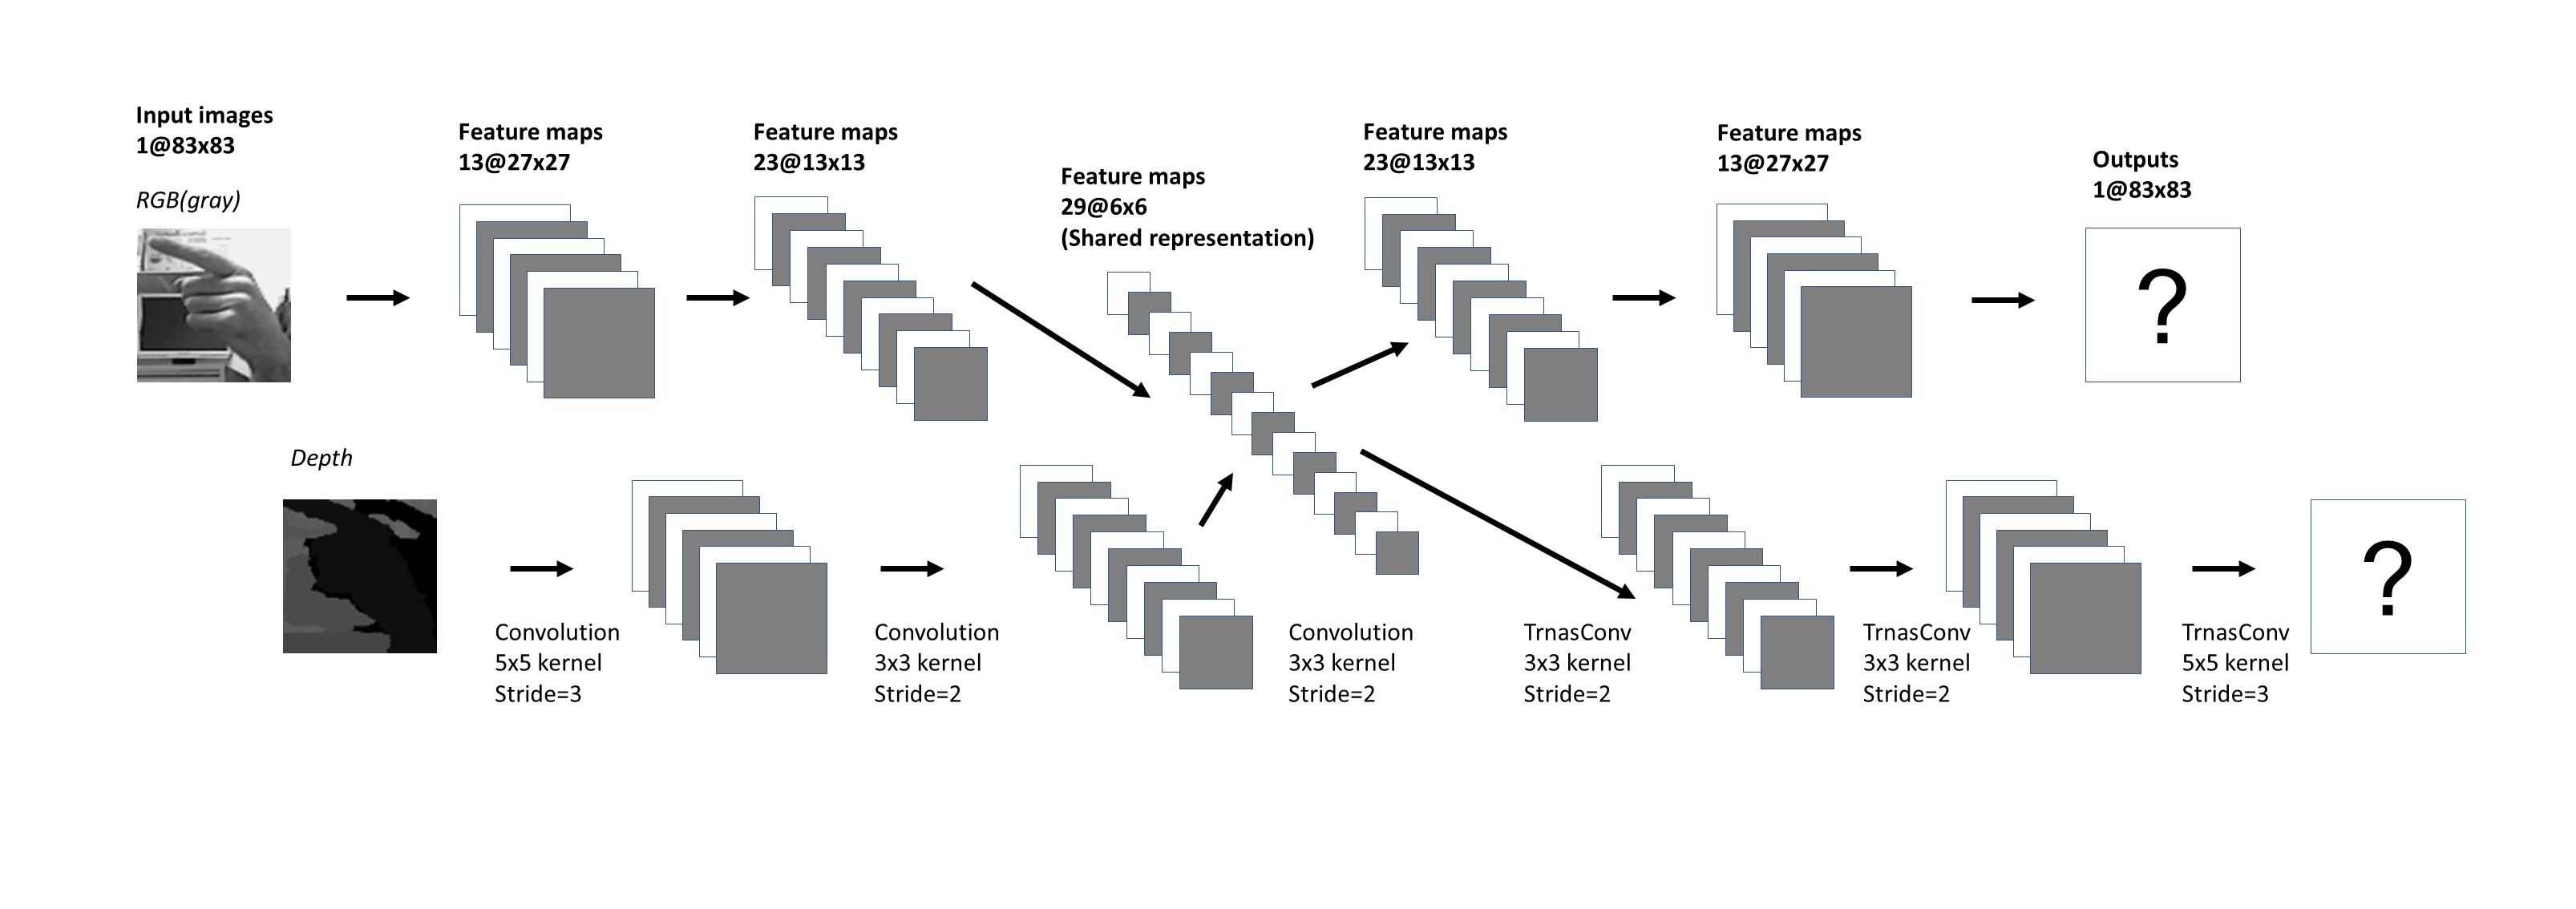
\includegraphics[width=0.95\linewidth]{architectures/FAE5}
  \caption{%
    \textbf{The bimodal convolutional auto-encoder model that is
      used to learn shared multimodal representation.}\\[0.1em]
    We simply take the CAE architecture that is introduced
      \autoref{fig:CAE5} for each modaliy but force them to have a
      shared middle layer by adding the corresponding activation values.
      We then try to reconstruct the two images separately through
      two disjoint paths.}
  \label{fig:FAE5}
\end{figure}

Ideally, we expect that the network is able to capture corrlations
across different modalities and can thus also learn a better single
modality representation. To verify this hypothesis, I built a perceptron
on the top of the middle layer of the architecture and trained it
in a supervised way while only one modality was given in input. For example,
if I wanted to train a classifier for color images, zeros were fed as
depth inputs. The results are shown in \autoref{tab:ASL_classif}.
Unfortunately, the presence of the two modalities during feature
learning doesn't bring a significant improvement and seems to be useless.

How about exploiting the information from the two modalities in a
totally supervised way? I took the CNN architecture of \autoref{fig:CNN10}
for color and depth images separately until the seventh layer where
a fusion was carried out. After training the network, the prediction
accuracy was always at about 80\% and no improvement was obtained compared
with a CNN trained only on color inputs. To conclude, color and depth
images are probably two modalities that are too similar. Color images
contain already all the necessary information for the task at hand so
that depth maps don't bring any supplementary information that benefit
the specifique purpose I defined.

However, multimodal information may still be useful when one or several
modalities are noisy whereas clean information are available for the others.
For example, I trained a network to construct clean color images from
noisy depth maps. When I did the classification based on the learned
representation, the performance was as if I trained directly a depth CAE.

\begin{table}[H]
  \tabcolsep = 9pt
  \caption{\textbf{Classification performance on the ASL Finger Spelling
    dataset}\\[0.1em]
    Raw) Perceptron that reads raw input data.\\[0.1em]
    CAE features) Perceptron stacked on the middle layer of the CAE.
      (\ref{subsection:CAE}).\\[0.1em]
    Shared) Perceptron that exploits the shared representation learned
      by a bimodal CAE (\ref{subsection:shared}).\\[0.1em]
    CAE architecture) Perceptron stacked on the middle layer of the CAE
      but train the whole network in a supervised way as a CNN.\\[0.1em]
    CNN) The CNN architecture in \autoref{fig:CNN10}
      (\ref{subsubsection:ASL_CNN}). \\[0.1em]
    The used hyperparameters are $\alpha_0=0.005$, $\gamma=0.8$ and
    $\eta=0.0004$. We notice that we have exactly the same network
    architecture for the middle three exerimental setups and only the
    training process differs one from another.
    }
  \label{tab:ASL_classif}
  \begin{tabular*}{\linewidth}{>{\bf}llccccc}
    \toprule
    && Raw & CAE features & Shared & CAE architecture & CNN\\
    \midrule
    \multirow{2}{*}{Intensity} &
    train & 69.47 \% & 78.87 \% & 85.85 \% & 91.29 \% & 99.69 \% \\
    & test & 32.64 \% & 50.24 \% & 53.38 \% & 65.44 \% & 79.73 \% \\
    \midrule
    \multirow{2}{*}{Depth} &
    train & 63.64 \% & 79.61 \% & 81.83 \% & 88.80 \% & 97.24 \% \\
    & test & 29.93 \% & 41.64 \% & 42.85 \% & 55.62 \% & 64.46 \% \\
    \bottomrule
  \end{tabular*}
\end{table}

We may also want to ask if this architecture, when a partial input with
only one modality is given, is able to infer the values of the missing
modality.
Several examples can be seen in \autoref{fig:color_depth_restoration}.
Visually speaking, the reconstruction result seems better when
both modalities are available in input even though they're both very noisy.
Knowing that the two modalities are already quite similar, it reveals
the difficulty of this task and the problem of multimodal retrieval
might be something that is more insteresting than trying to construct
information of some modality from zero.

\begin{figure}[H]
  \centering
  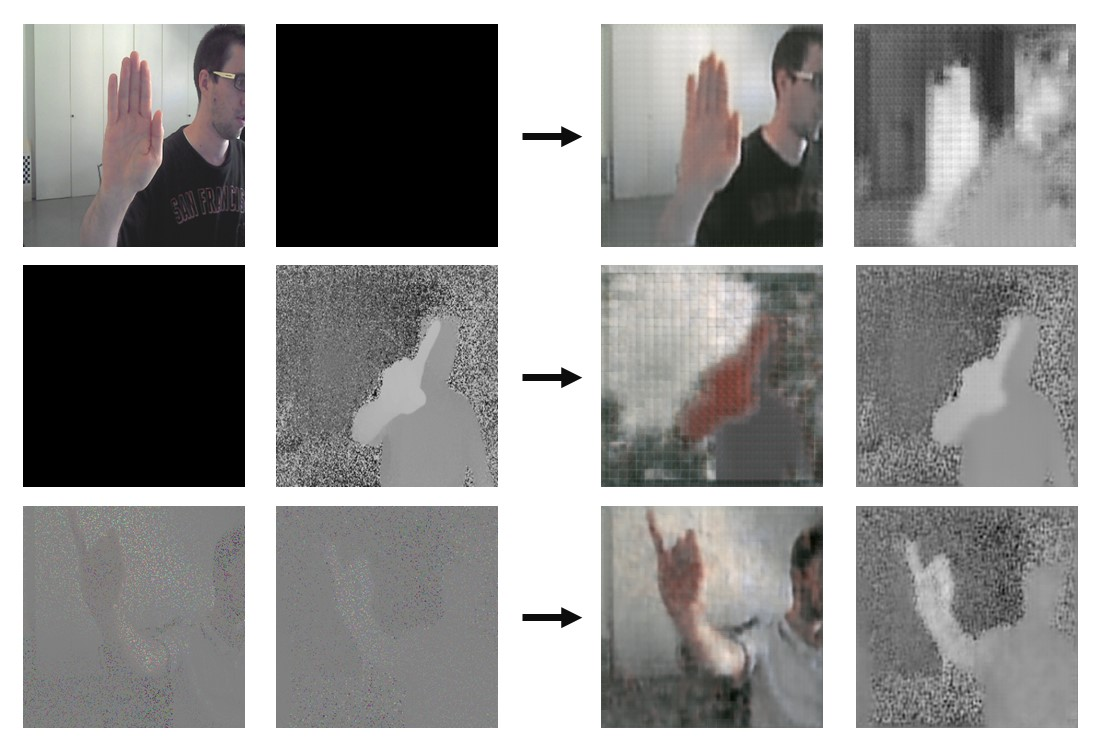
\includegraphics[width=\linewidth]{dataset/senz3d/reconstructions}\\[-1em]
  \caption{%
    \textbf{Restore color and depth images from incomplete input
      information.}\\[0.1em]
    Top) Only the color image is given.\\[0.1em]
    Middle) Only the depth image is given.\\[0.1em]
    Botttom) Both modalities are given but with little information
      (10\% of pixels).}
  \label{fig:color_depth_restoration}
\end{figure}

\subsection{Transfer learning} \label{subsection:AVSR_transfer}

In the second part of this section, we'll discuss the knowledge transfer
problem between different modalities. This work was very similar to what
had been done in \cite{S. Moon 2015}, but at the same time it can also be
viewed as a form of zero-shot learning \cite{A. Frome 2013, R. Socher 2013}.

I studied particularly the transfer between speech and lip-reading
video data using the AVLetters dataset. First the dataset was separated
randomly into two parts, which I'll still call training and test set
by an abus of language. They're respectively noted $Tr$ and $Te$.
$Tr$ contained 600 data samples while $Te$ comprised the left 180 instances.
For $X$ an arbitrary subset of data, $X^a$ and $X^v$ denote respectively
the audio and video data in $X$.

Next, to simulate the imbalance of data quantity between different
modalities in the real world, I further splitted $Tr$, $Te$ into
$Tr_{A\sim T}$, $Tr_{U\sim Z}$, $Te_{A\sim T}$ and $Te_{U\sim Z}$
according to the label of each sample.
For instance, a lip-reading video of a speaker saying E is in either
$Tr_{A\sim T}^v$ or $Te_{A\sim T}^v$.
During the first training stage, the video model was only accessible
to a partial label space. The network was trained on $Tr_{A\sim T}^v$
which contained 466 samples. On the other hand, the audio model was trained
on the whole label space $Tr^a$.

Next, I wanted to leverage speech data to fine-tune the network trained for
video recognition. For a data sample $x^a\in Tr_{U\sim Z}^a$, I first
computed its audio representation $h^a(x^a)$ that was taken from some
hidden layer of audio model. A transfer funcion $\mathcal{T}$ was used
to approximate the video representation of this data sample.
That is, we want $\mathcal{T}(h^a(x^a))\approx h^v(x^v)$. Finally, I
fine-tuned the subnetwork situated after the hidden video layer that
was taken as representation via a standard backpropagation algorithm.

The detailed experiement is presented in \autoref{fig:AVSR_transfer}.
For both audio and video network I chose the second hidden layer for
transfer. For the sake of simplicity, an instance-based approach
(KNN-based mapping) was employed to define $\mathcal{T}$.
I obtained mapping of a new audio
input $x^v$ by first finding the $K$-closest audio samples of
$Tr_{A\sim T}^a$ in the representation space, and then returning the
average values of the corresponding video samples
(also in the representation space).

\begin{figure}[H]
  \centering
  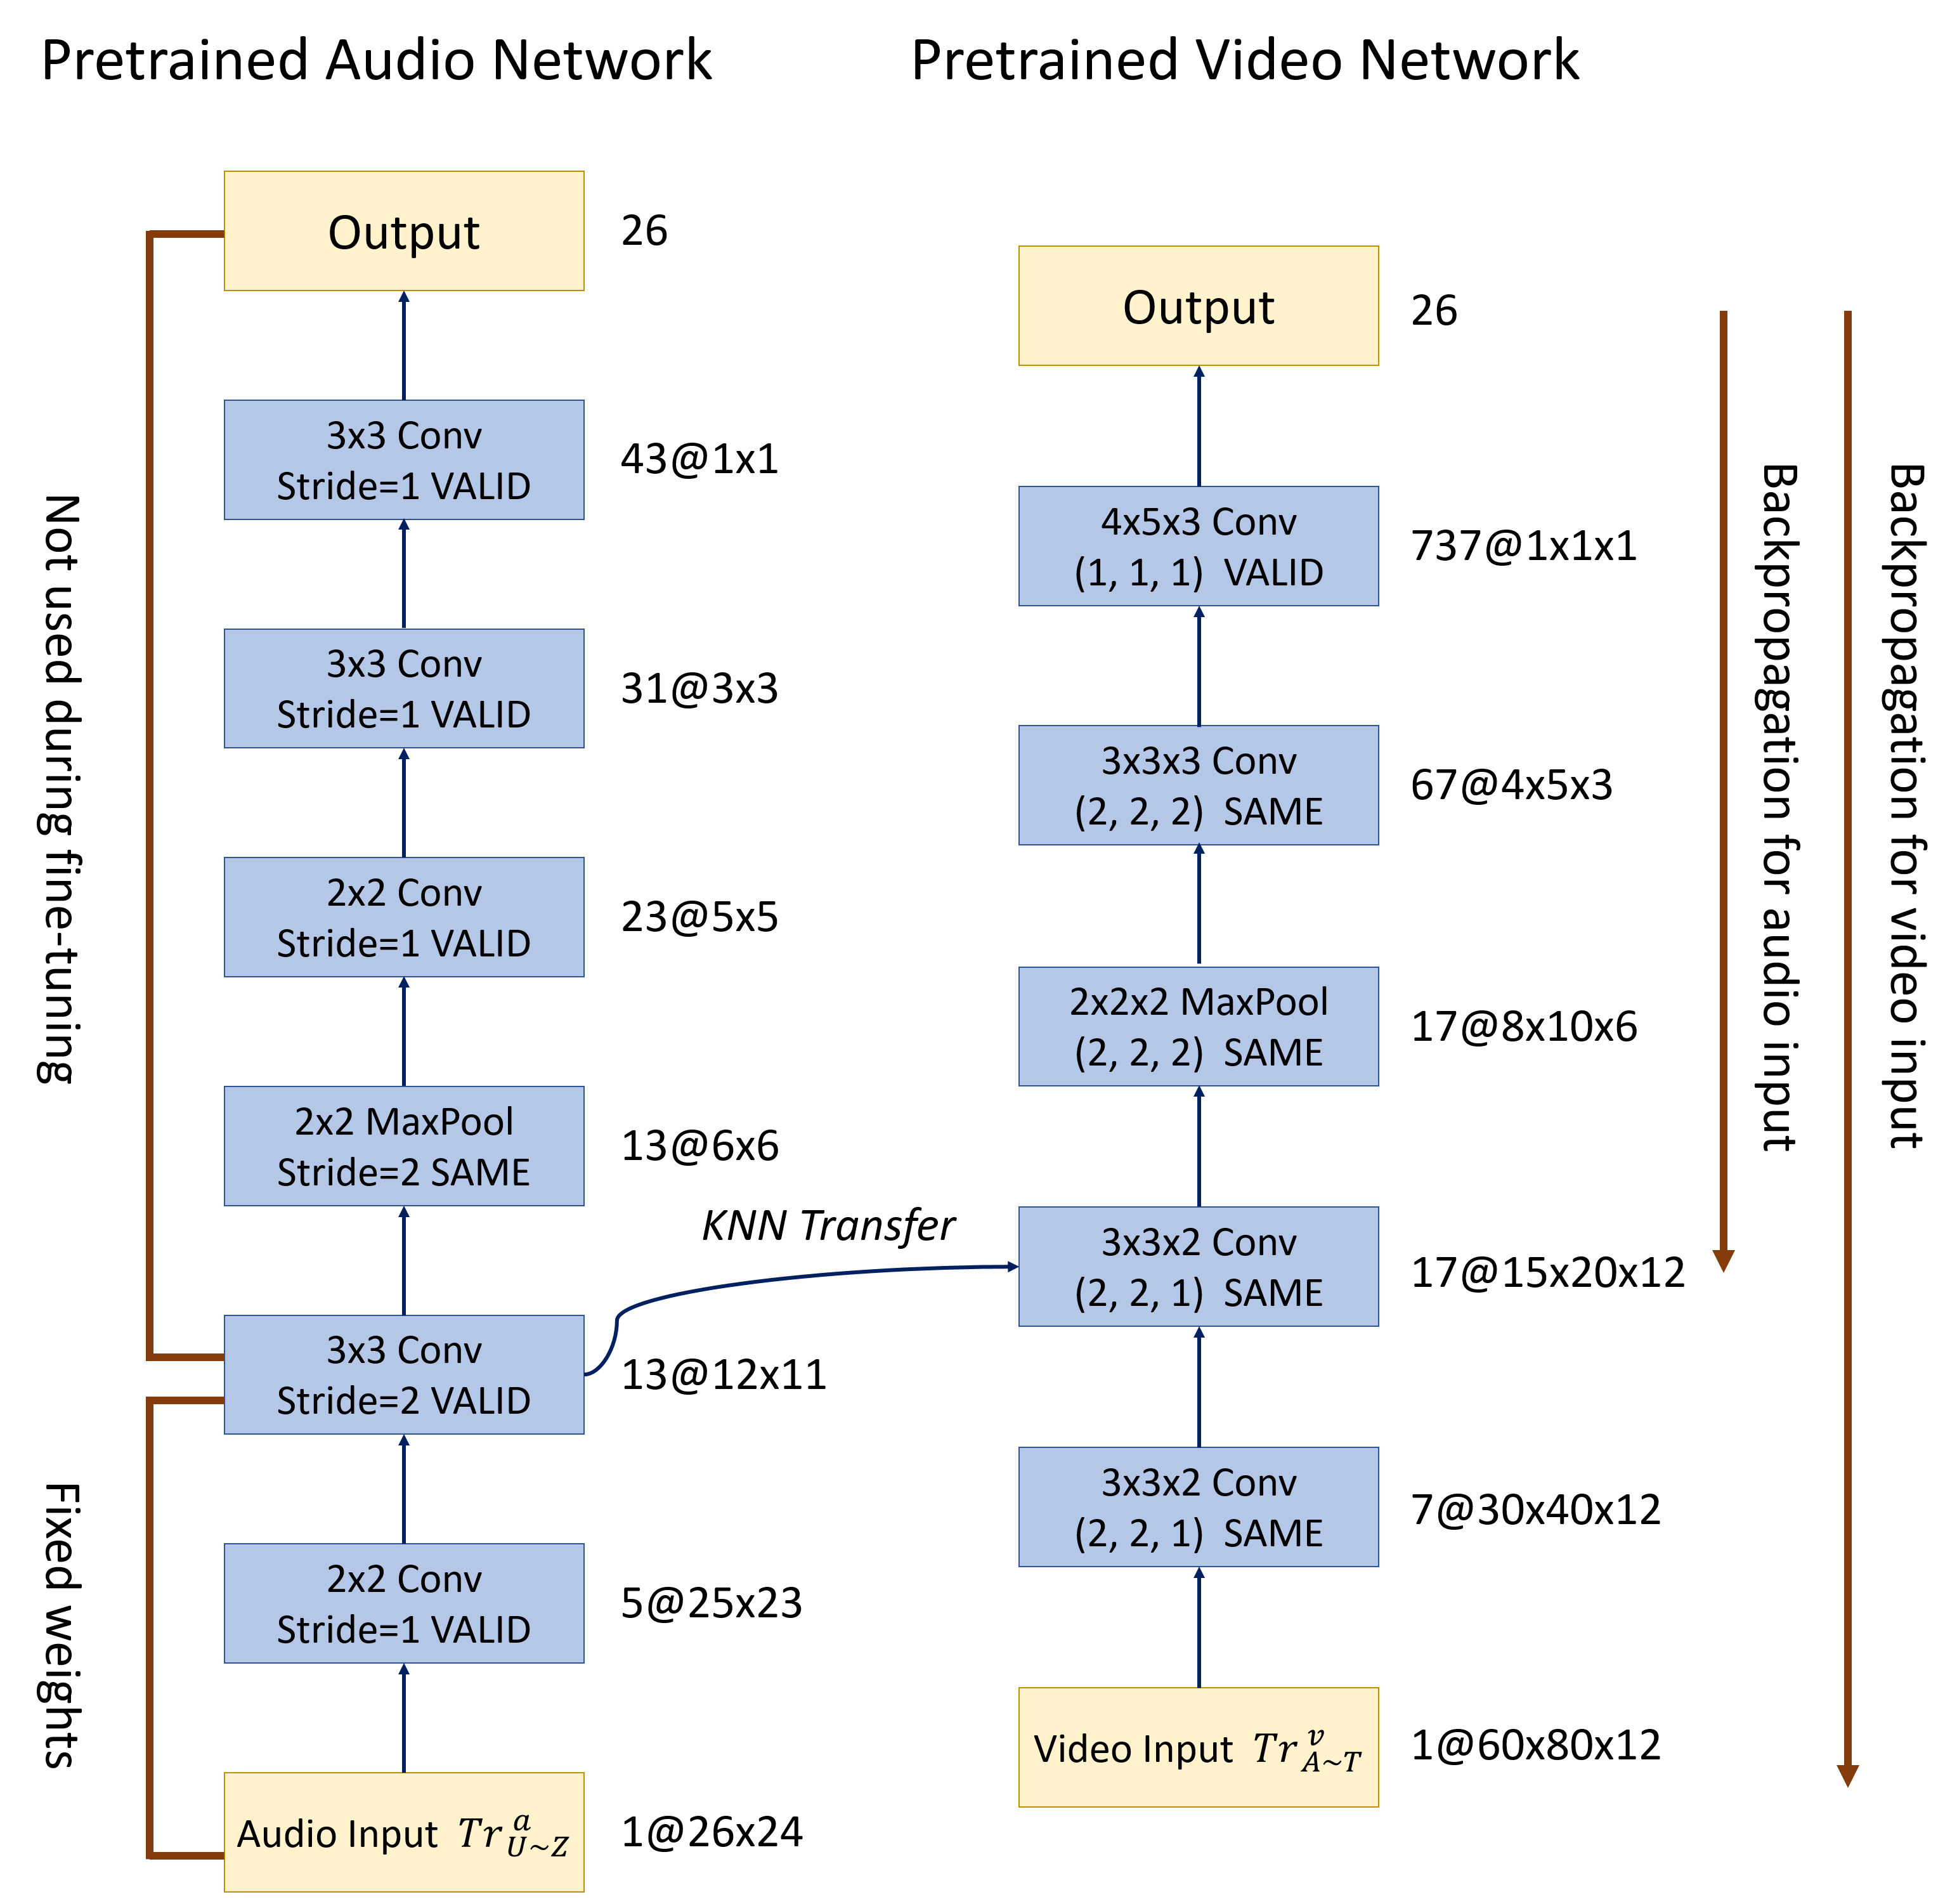
\includegraphics[width=0.9\linewidth]{architectures/AVSR_transfer}
  \caption{%
    \textbf{Illustration of the transfer learning approach applied in
      audio and lip-reading speech recognition tasks.}\\[0.1em]
    We first learn two separated model for audio and visual inputs
      (in my cases two CNNs) and try to fine-tune the video network
      with transferred audio data.
    }
  \label{fig:AVSR_transfer}
\end{figure}

Nonetheless, if only audio inputs were presented during fine-tuning, it
might cause a bias of the fine-tuned network towards the six new classes.
To avoid this problem, data from $Tr_{A\sim T}^v$ were also fed as input
from time to time to fine-tune the whole network. Concretely, with
probability $p_a$ audio data was presented and otherwise video input
was given. At the end, the new network was tested on different parts of
video data for evaluataion.

Many experiments with various hyperparameter values were conducted
and some results are shown in \autoref{tab:AVSR_transfer}.
We see that despite the fact that the overall performance isn't improved
by knowledge transfer, the fine-tuned network is now able to classify
samples whose labels range from U to Z with an accuracy of 10-20\%
(\textbf{Exp1}). It shows the utility of the transfer learning approach
although there is still a long way to go before it becomes
useful in practice.
During fine-tuning, the magnitude of learning rate is equally important.
As we can see, if the learning rate is too high, it can deteriorate
the pre-trained network and the performance may drop drastically
(\textbf{Exp2}).
On the other hand, as predicted before, if only audio data labeled from
U to Z are provided for fine-tuining, the classification performance
drops for the first twenty labels even though a higher accuracy (40-50\%)
can be achieved for the last six labels (\textbf{Exp3}).
We also observe that there isn't a great difference when the network is
tested on $Tr_{A\sim T}^v$ or $Te_{A\sim T}^v$.

\begin{table}[H]
  \tabcolsep = 13pt
  \caption{\textbf{Some results of the audio-visual transfer experiment.}
    \\[0.1em]
  The audio model was pre-trained with $\eta=0.1$, $\alpha_0=0.005$ and
  $\gamma=0.8$ while the video model was pre-trained with $\eta=0.0004$,
  $\alpha_0=0.002$ and $\gamma=0.96$. The transfer learning experiment
  was carried out under the setting $\eta=0.0004$, $\gamma=0.8$, $K=12$
  and was trained for 160 steps.
  For \textbf{Exp1}, \textbf{Exp2} and \textbf{Exp3}, I used respectively
  $\alpha_0 = 0.001, 0.005, 0.001$ and $p_a = 0.85, 0.85, 1$.
  }
  \label{tab:AVSR_transfer}
  \begin{tabular*}{\linewidth}{>{\bf}lcccccc}
    \toprule
    & $Tr^v$ & $Tr^v_{A\sim T}$ & $Tr^v_{U\sim Z}$
    & $Te^v$ & $Te^v_{A\sim T}$ & $Te^v_{U\sim Z}$\\
    \midrule
    No transfer & 77.67 \% & \textbf{100} \% & 0 \% & \textbf{40.56} \%
    & \textbf{54.48} \% & 0 \% \\
    Exp1 & \textbf{81.17} \% & 98.28 \% & 21.64 \% & 39.44 \%
    & 47.76 \% & 15.22 \% \\
    Exp2 &  40.83 \% & 51.07 \% & 5.22 \% & 23.89 \%
    & 30.60 \% & 4.35 \% \\
    Exp3 & 19.67 \% & 12.23 \% & \textbf{45.52} \% & 12.22 \%
    & 2.24 \% & \textbf{41.34} \% \\
    \bottomrule
  \end{tabular*}
\end{table}

\section{Conclusion and Perspective} \label{section:conclusion}

In this report, I have introduced two different multimodal learning
settings and evaluated them on three different datasets.
However, no significant results were obtained for the shared
representation learning experiment and the knowledge transfer experiment
aroused only moderate interest.
Several possible reasons should be mentioned.
First, the used datasets may be too small and monotonous and
prevent the network from learning a good representation of the data.
Second, since I didn't do an intense study in the domain of
representation learning and dimension reduction, the algorithms
applied to single modality for extracting features may not be totally
adequate. Finally, the proposed experiments might be in essence
inappropriate for some configurations. For example, depth maps may be
redundant when color images are already present.

In spite of this, my work still ensured the possiblity and the possible
benefit of taking into multiple modalities into account while
dealing with real world problems. This needs to be further studied
with better representation learning algorithms and bigger datasets.
Ideally, we should try to apply these techniques to real
data coming from human-robot interactions to see if it's possible
to make the robot's behavior more humanlike thanks to multimodal fusion.
On the other hand, there are still many multimodal learning models
to be explored. For instance, we can project features from different
sources into a joint space while trying to minimizing the distance
between modalities (this is called a ``coordinated representation''
in \cite{T. Baltrusaitis 2017}). I have worked a little on similar
experiments but the difficulty consists in finding the appropriate
loss function.



%14 22 46
